%%%%%%%%%%%%%%%%%%%%%%%%%%%%%%%%%%%%%%%%%%%%%%%%%%%%%%%%%%%%%%%%%%%%%%%%
%
%
%     This file is included from the file   Segmentation.tex
% 
%     Section tag and label are placed in this top file.
%
%
%
%%%%%%%%%%%%%%%%%%%%%%%%%%%%%%%%%%%%%%%%%%%%%%%%%%%%%%%%%%%%%%%%%%%%%%%%

\subsection{Introduction}
\label{sec:HybridSegmentationIntroduction}
  This section introduces the use of hybrid methods for segmentation
of radiological patient data and the Visible Human data. The hybrid
segmentation approach integrates boundary-based and region-based
segmentation methods that amplify the strength but reduce the
weakness of both approaches. The advantage of this approach comes
from combining region-based segmentation methods like the fuzzy
connectedness and Voronoi diagram classification with boundary-based
deformable model segmentation. The synergy between fundamentally
different methodologies tends to result in robustness and higher
segmentation quality.  A hybrid segmentation engine can be built, as
illustrated in
Figure\ref{fig:ComponentsofaHybridSegmentationApproach}. It consists
of modules representing segmentation methods (ITK filters). We can
derive a variety of hybrid segmentation methods by exchanging the
filter use in each module. It should be noted that under the fuzzy
connectedness and deformable models modules, there are several
different filters that can be used as components. Below, we describe
two examples of hybrid segmentation methods, derived from the hybrid
segmentation engine: integration of fuzzy connectedness and Voronoi
diagram classification (hybrid method 1), and integration of Gibbs
prior and deformable models (hybrid method 2).  Details on the
concepts behind these methods have been discussed in the literature
\cite{Angelini2002,Udupa2002,Jin2002,Imielinska2001,Imielinska2000a,Imielinska2000b}



\subsection{FuzzyConectedness and VoronoiDiagramClassification}
\label{sec:HybridMethod1}
 In this section, we present a hybrid segmentation method that
requires minimal manual initialization, where we integrate the fuzzy
connectedness Segmentation and Voronoi diagram Classification. We
start with a fuzzy connectedness filter to generate a sample of
tissue from a region to be segmented. From the sample, we
automatically derive homogeneity statistics that constitute the
homogeneity operator to be used in the next stage of the method. The
output of the fuzzy  connectedness filter is used as a prior for the
Voronoi diagram classification  filter that performs iterative
subdivision and classification of the segmented image that results in
an estimation of the boundary. The output of this filter is a 3D
binary image that can be used to display the 3D result of the
segmentation, or passed to another filter (e.g. deformable model) for
further improvement of the final segmentation. Details describing the
concepts behind these methods  have been published in
\cite{Angelini2002,Udupa2002,Jin2002,Imielinska2001,Imielinska2000a,Imielinska2000b}

In Figure \ref{fig:UMLClassDiagramoftherFuzzyConnectednessFilter}, we describe 
the base class for simple fuzzy connectedness segmentation. This method is non-scale 
based and non-iterative, and requires only one seed to initialize it. We define affinity 
between two nearby elements in a image (e.g. pixels, voxels) via a degree of adjacency, 
similarity of their intensity values, and their similarity with the estimated object. 
The closer the elements and the more similar their intensities, the greater the affinity between them. We compute the strength of a path and fuzzy connectedness 
between each two pixels (voxels) in the segmented image from the fuzzy affinity. 
Computation of the fuzzy connectedness value of each pixel (voxel) is implemented
by selecting a seed point and using dynamic programming. The result constitutes the fuzzy
map. Thresholding of the fuzzy map gives a segmented object that is strongly connected
to the seed point (for more details, see \cite{Udupa1996}). We checked in two fuzzy 
connectedness filters: the \code{itkSimpleFuzzyConnectednessScalarImageFilter}, an
implementation of the fuzzy connectedness segmentation of single-channel (grayscale) 
image, and the \code{itkSimpleFuzzyConnectednessRGBImageFilter}, an implementation of fuzzy
connectedness segmentation of a three-channel (RGB) image. Other classes can be derived 
from the base class by defining other affinity functions and targeting multi-channel
images with an arbitrary number of channels. It has to be noted that the simple fuzzy 
connectedness filter can be used as a stand-alone segmentation method,
as described in the diagram in Figure 
\ref{fig:UMLCollaborationDiagramoftheFuzzyConnectednessFilter}.

In Figure \ref{fig:UMLVoronoiSegmentationClassFilter} we present the base class for
Voronoi diagram classification. We initialize the method with a number of random
seed points and compute the Voronoi diagram over the segmented 2D image. Each
Voronoi region in the subdivision is classified as internal or external,
based on the homogeneity operator derived from the fuzzy connectedness
algorithm.  We define boundary regions as the external regions that are
adjacent to the internal regions.  We further subdivide the boundary regions
by adding seed points to them. We converge to the final segmentation
using simple stopping criteria (for details, see \cite{Imielinska2001}). We
implemented two Voronoi diagram filters: the
\code{itkVoronoiSegmentationImageFilter}, dedicated to processing single-channel
(grayscale) images, and the \code{itkVoronoiSegmentationRGBImageFilter}, that segments
three-channel (RGB) images. Other classes can be derived from the base class
by defining other homogeneity measurements and targeting multichannel images
with an arbitrary number of channels.  The other classes that are used for
computing a 2D Voronoi diagram are shown in Figure
\ref{fig:UMLClassesforImplementationofVoronoiDiagramFilter}. We note that the
Voronoi diagram filter can be used as a stand-alone segmentation method, as
depicted in Figure
\ref{fig:UMLCollaborationDiagramoftheVoronoiSegmentationFilter}.

 We present diagrams in Figures \ref{fig:UMLHybridMethodDiagram1} and 
 \ref{fig:UMLHybridMethodDiagram2} for hybrid segmentation methods
 that integrate fuzzy connectedness with Voronoi diagrams, and fuzzy
 connectedness, Voronoi diagrams and deformable models, respectively.


\begin{figure}
\center
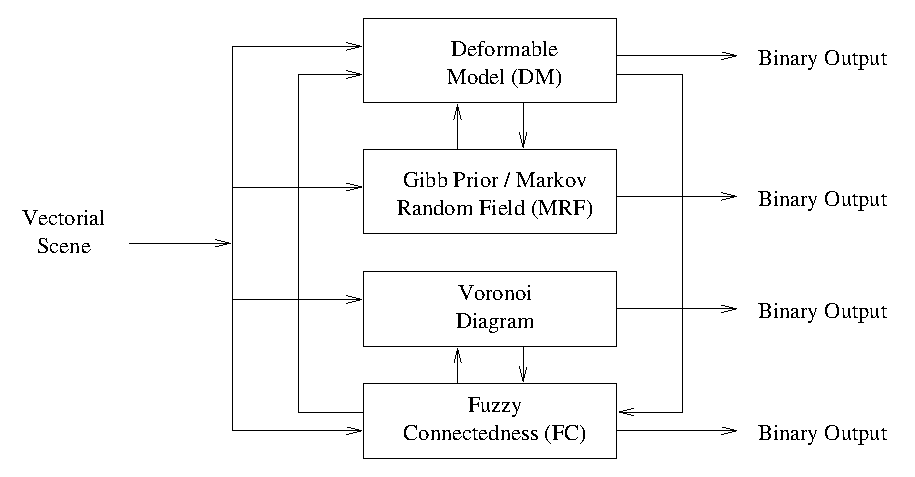
\includegraphics[width=14cm]{HybridSegmentationEngine1.eps}
\itkcaption[Hybrid Segmentation Engine]{Hybrid Segmentation Engine}
\label{fig:ComponentsofaHybridSegmentationApproach}
\end{figure}


\begin{figure}
\center
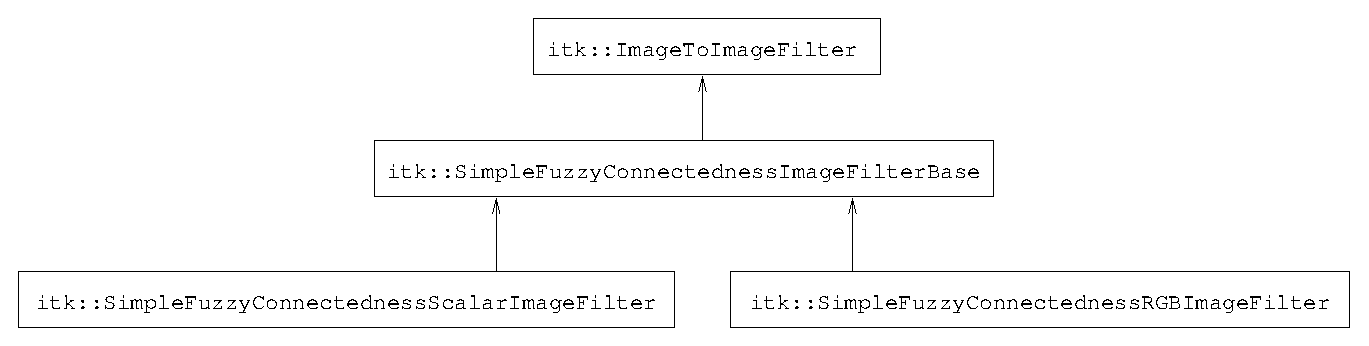
\includegraphics[width=14cm]{FuzzyConnectednessClassDiagram1.eps}
\itkcaption[FuzzyConectedness Filter Diagram]{Diagram of the FuzzyConnectedness filter}
\label{fig:UMLClassDiagramoftherFuzzyConnectednessFilter}
\end{figure}


\begin{figure}
\center
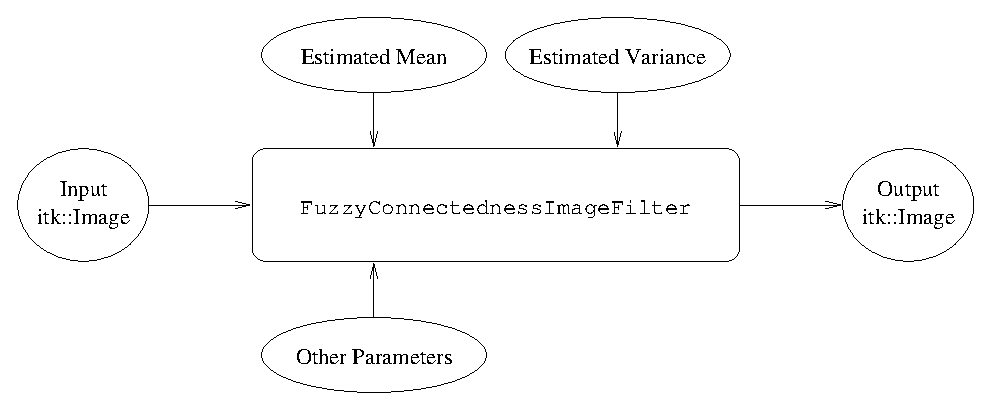
\includegraphics[width=14cm]{FuzzyConnectednessCollaborationDiagram1.eps}
\itkcaption[Fuzzy Connectedness Segmentation Diagram]{Diagram Of Stand-Alone
Fuzzy Connectedness Segmentation}
\label{fig:UMLCollaborationDiagramoftheFuzzyConnectednessFilter}
\end{figure}

\begin{figure}
\center
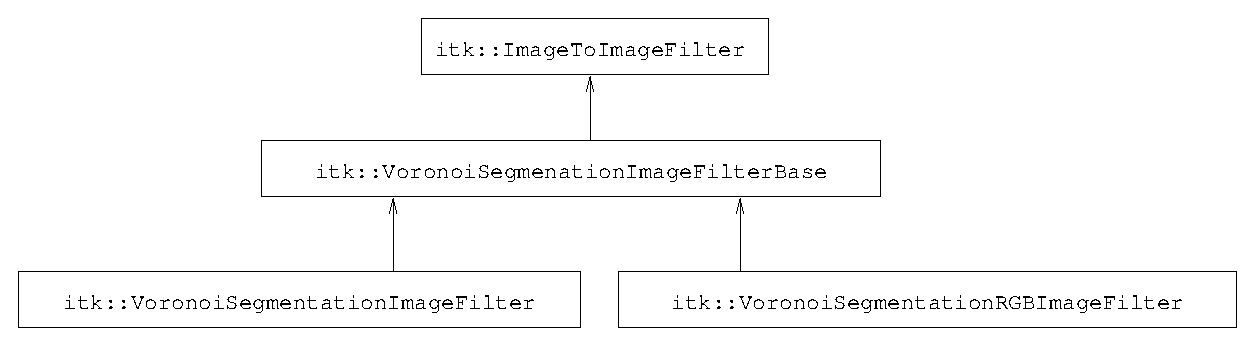
\includegraphics[width=14cm]{VoronoiSegmentationClassDiagram1.eps}
\itkcaption[Voronoi Filter class diagram]{Diagram of the Voronoi Diagram Classification filter}
\label{fig:UMLVoronoiSegmentationClassFilter}
\end{figure}

\begin{figure}
\center
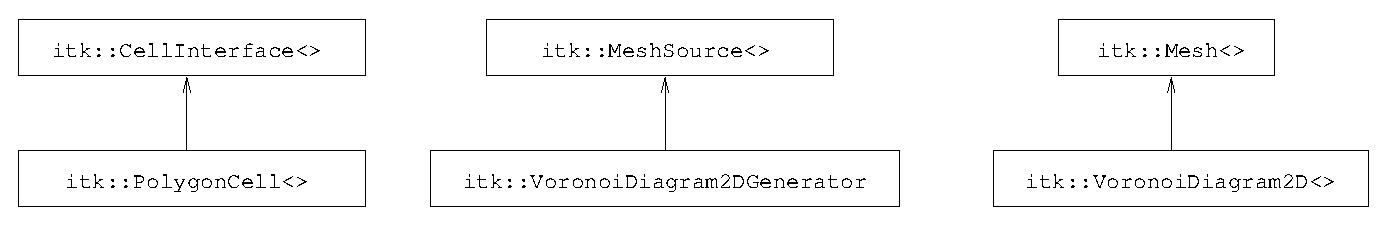
\includegraphics[width=14cm]{VoronoiSegmentationCollaborationDiagram1.eps}
\itkcaption[Voronoi Diagram Filter classes]{Classes for Implementation of Voronoi Diagram Filter}
\label{fig:UMLClassesforImplementationofVoronoiDiagramFilter}
\end{figure}


\begin{figure}
\center
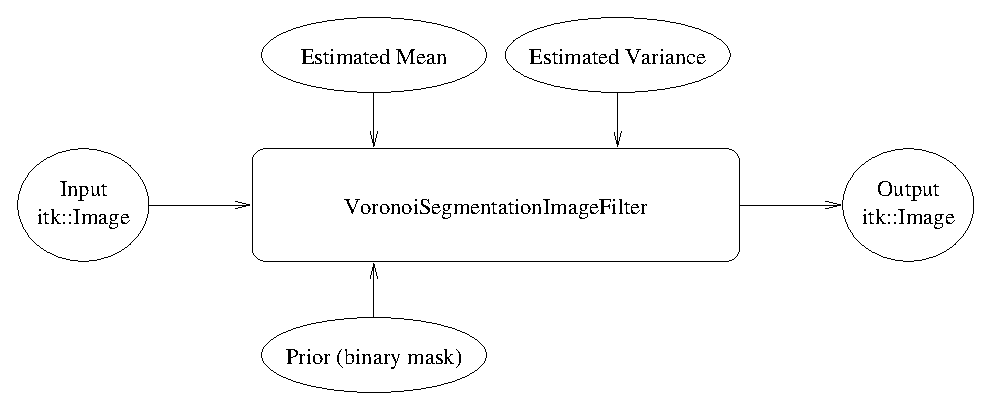
\includegraphics[width=14cm]{VoronoiSegmentationCollaborationDiagram2.eps}
\itkcaption[Voronoi Diagram Segmentation]{Diagram Of Stand-Alone Voronoi Diagram Segmentation}
\label{fig:UMLCollaborationDiagramoftheVoronoiSegmentationFilter}
\end{figure}


\begin{figure}
\center
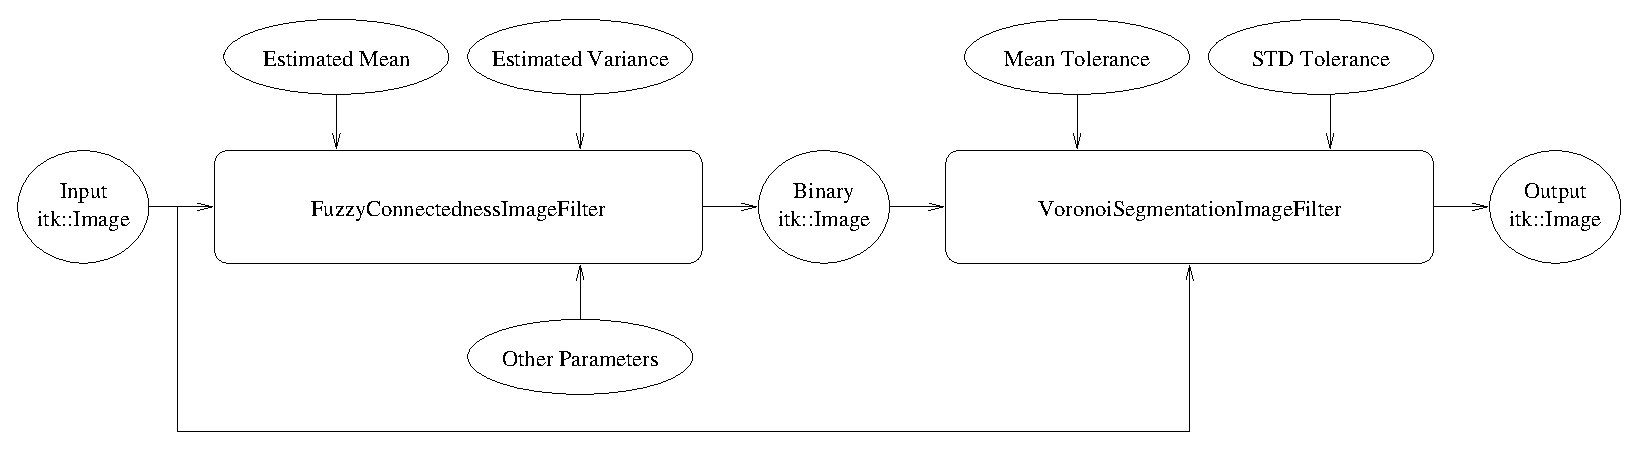
\includegraphics[width=14cm]{FuzzyVoronoiCollaborationDiagram1.eps}
\itkcaption[Fuzzy Connectedness and Voronoi Diagram Classification]{Integration of
Fuzzy Connectedness with Voronoi Diagram Classification}
\label{fig:UMLHybridMethodDiagram1}
\end{figure}

\begin{figure}
\center
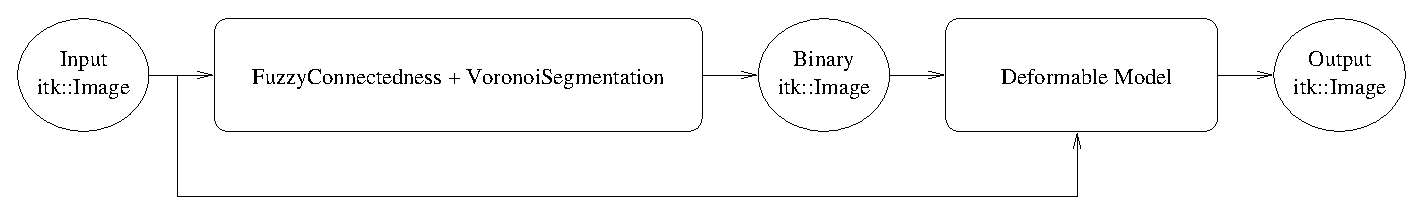
\includegraphics[width=14cm]{FuzzyVoronoiDeformableCollaborationDiagram1.eps}
\itkcaption[Fuzzy Connectedness, Voronoi diagram, and Deformable
Models]{Integration of Fuzzy Connectedness, Voronoi diagram, and Deformable
Models}
\label{fig:UMLHybridMethodDiagram2}
\end{figure}



\subsubsection{Example of a Hybrid Segmentation Method}
\label{sec:HybridMethod1:Example}

\ifitkFullVersion
\input{HybridSegmentationFuzzyVoronoi.tex}
\fi



\subsection{Deformable Models and Gibbs Prior}

Another combination that can be used in a hybrid segmentation method is the
set of Gibbs prior filters with deformable models.

\subsubsection{deformable model}
\ifitkFullVersion
\input{DeformableModel1.tex}
\fi


\subsubsection{Gibbs Prior Image Filter}
\ifitkFullVersion
\input{GibbsPriorImageFilter1.tex}
\fi

